\chapter{Compact Muon Solenoid}

\section{scratch}
Mention the location of CMS.  Give an overview of what it was designed to do.  Find a nice way to say that there is a lot of shit coming from the interaction region and we have to sort through it.  We need to get charged particle momentum and energy, electromagnetic energy, 

\section{Introduction}
About 100 meters below the town of Cessy, France at Point 5 is the Compact Muon Solenoid (CMS).  The CMS is a general purpose detector weighing 14,000 tonnes with a length of 28.7 meters and a 15.0-meter diameter that was designed to accurately measure the energy and momentum of particles produced in the proton-proton or heavy-ion collisions at the LHC \cite{Collaboration_2008}.  A perspective view of of the detector is shown in Figure \ref{fig:cmsschematic}.  In order to get a full picture of what is being produced by the collisions the CMS detector must be able identify the resulting particles as well as accurately measure their energy and momentum.  For this reason the detector was designed to be a collection of specialized sub-detectors, each of which contributes data used in the reconstruction of a collision.  
\begin{figure}[h]
	\centering
	\includegraphics[width=0.7\linewidth]{Figures/cms_schematic}
	\caption{Schematic of CMS detector \cite{Sakuma_2014}}
	\label{fig:cmsschematic}
\end{figure}

At the heart of the CMS detector is a 3.8-Tesla magnetic field produced by a superconducting solenoid.  Inside the 6-meter diameter solenoid are three layers of sub-detectors.  These make up the inner detector and are, in order from innermost to outermost, the silicon tracker, the electromagnetic calorimeter (ECAL), and the hadronic calorimeter (HCAL).  Outside the solenoid is the muon system.  A transverse slice of the detector (Figure \ref{fig:cmsslicewhitecolourfrench291016}) shows the sub-detectors and how different types of particles interact with with them.  Table \ref{table:subdetsignals} shows a summary of which sub-detectors are expected to produce signals for different types of particles.

\begin{figure}[h]
	\centering
	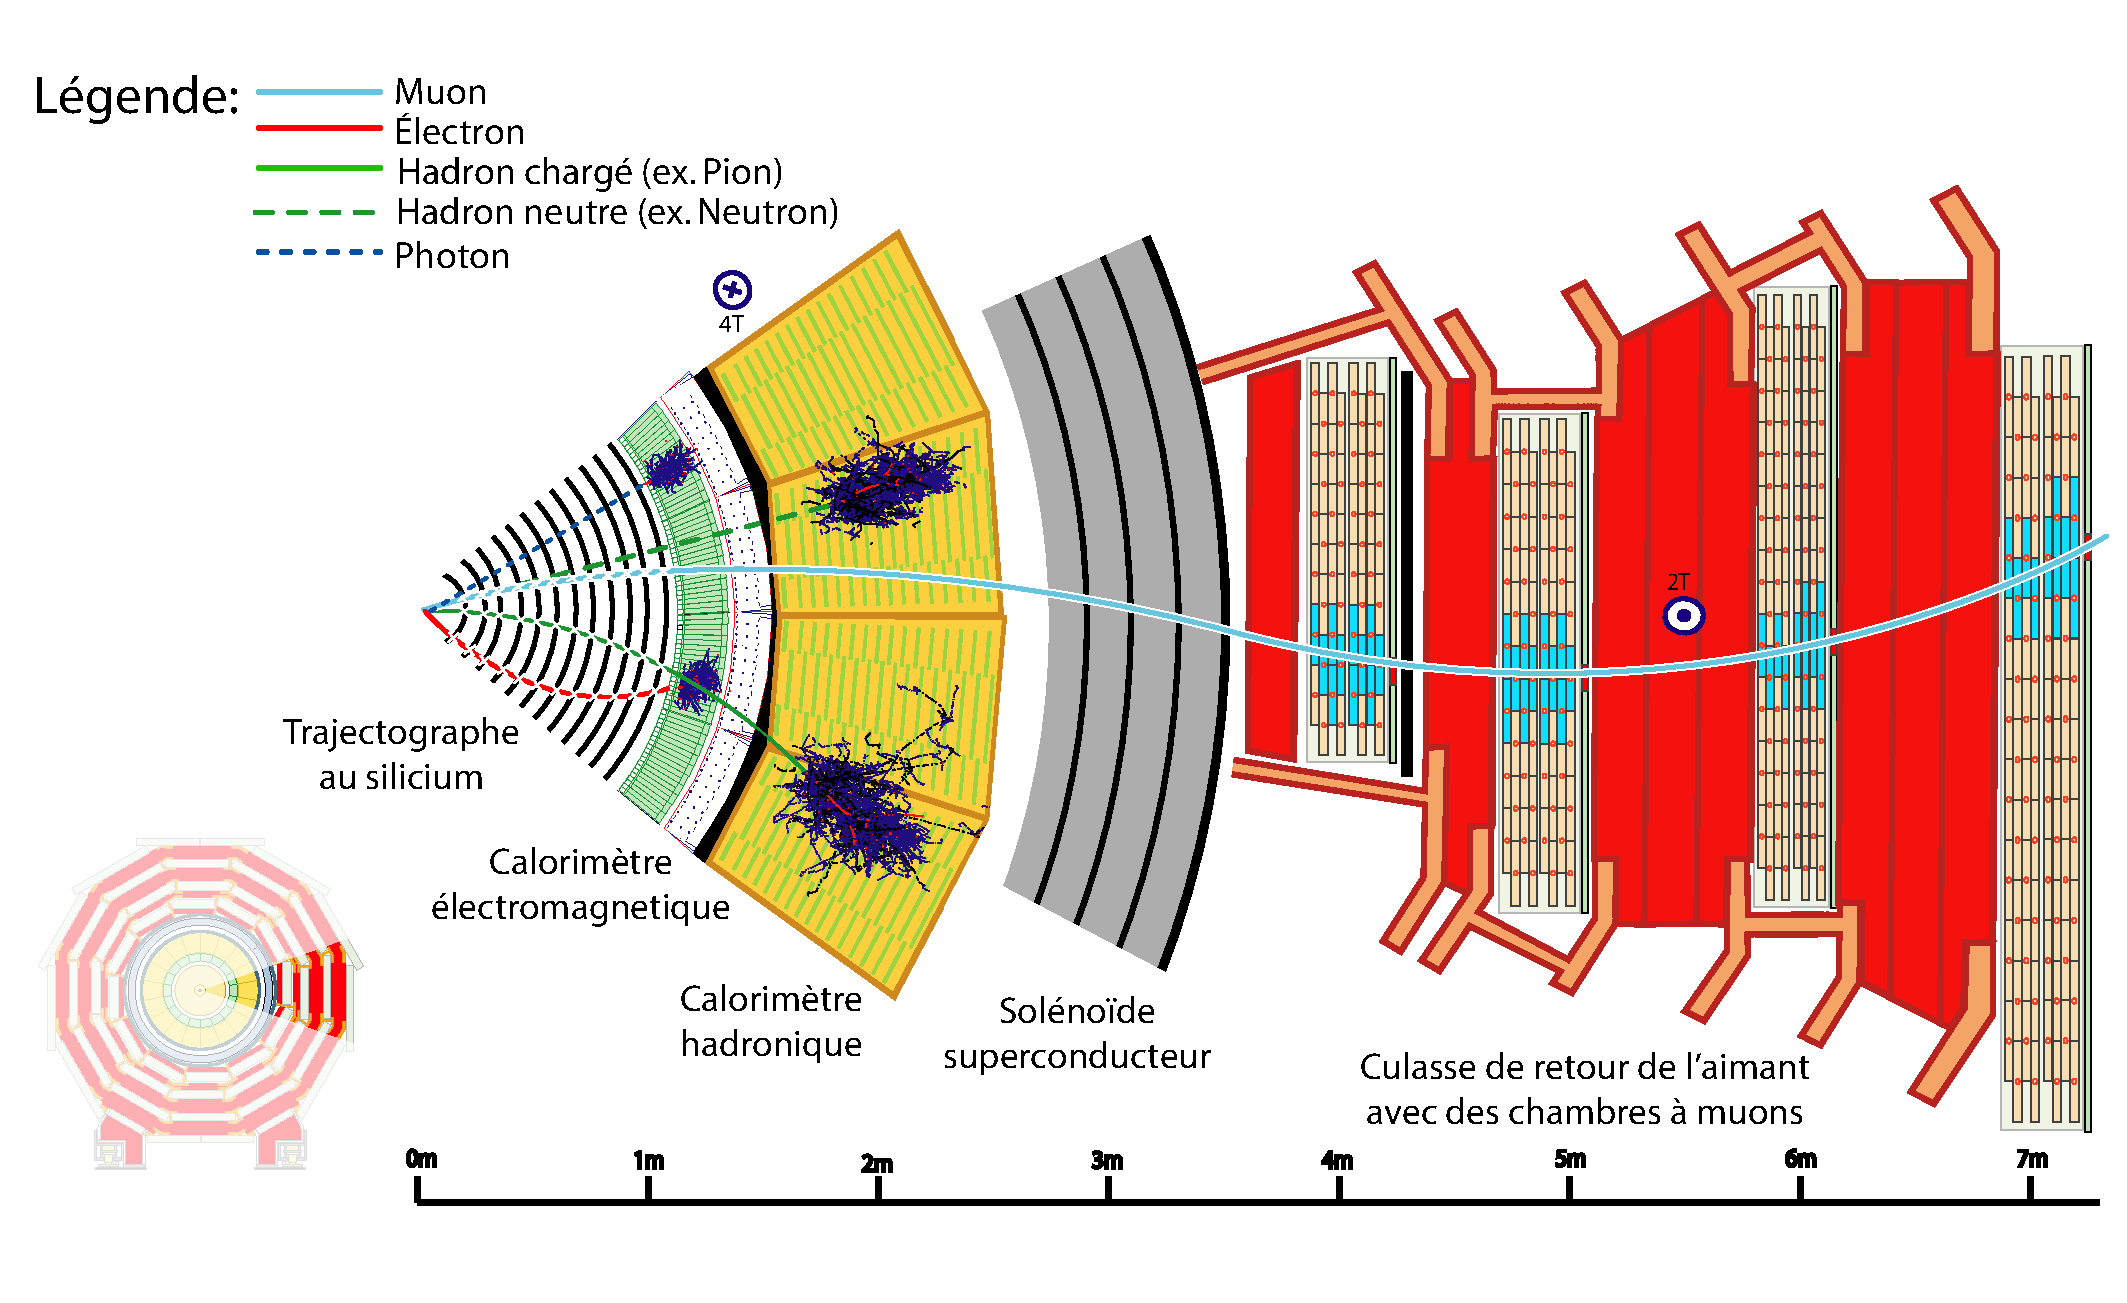
\includegraphics[width=0.7\linewidth]{Figures/CMS_slice_white_colour_french_291016}
	\caption{Transverse slice of the CMS detector\cite{Barney:2628641}.}
	\label{fig:cmsslicewhitecolourfrench291016}
\end{figure}



\begin{table}[h]
	\centering
\begin{tabular}{|c|c|c|c|c|}
	\hline 
	Particle & Tracker & ECAL & HCAL & Muon \\ 
	\hline 
	Photons & No & Yes & No & No \\ 
	\hline 
	Electrons & Yes & Yes & No & No \\ 
	\hline 
	Hadrons (charged) & Yes & No & Yes & No \\ 
	\hline 
	Hadrons (neutral) & No & No & Yes & No \\ 
	\hline 
	Muons & Yes & No & No & Yes \\ 
	\hline 
	Invisible ($\nu$, SUSY, etc) & No & No & No & No \\ 
	\hline 
\end{tabular} 
\caption{Summary of signals expected for each particle type in each sub-detector}
\label{table:subdetsignals}
\end{table}


\section{Coordinate System}
The origin of the coordinate system used by CMS is centered at the nominal collision point in the center of the detector.  A right-handed Cartesian system is used with the x-axis pointing radially inward toward the center of the LHC ring, y-axis pointing vertically upward, and the z-axis pointing tangent to the LHC ring in the counterclockwise direction as viewed from above.  CMS also uses an approximately Lorentz invariant spherical coordinate system spanned by three basis vectors.  They are the transverse momentum $p_{T}$, pseudorapidity $\eta$, and azimuthal angle $\phi$.  The transverse momentum and azimuthal angle translate to the Cartesian system in the following ways using the x and y-components of the linear momentum:
\begin{equation}
p_{T} = \sqrt{(p_{x})^{2} + (p_{y})^{2}}
\end{equation}
\begin{equation}
\phi = tan^{-1}\frac{p_{y}}{p_{x}}
\end{equation}
while the pseudorapidity can be translated using the polar angle $\theta$ relative the positive z-axis as
\begin{equation}
\eta = -ln[tan\frac{\theta}{2}].
\end{equation}

\section{Tracker}

\section{Electromagnetic Calorimeter}

\section{Hadronic Calorimeter}

\section{Muon System}

